In this project, the key idea is to convert an image classifier into an object detector. In particular, we explore a pre-trained ResNet50V2 CNN trained on the ImageNet dataset. Moreover, we make use of image pyramid and sliding windows.
Regarding image pyramid, it consists of different layers, each one representing an image at a different scale and usually a smoothing filter is applied. In our code, we implement  \textit{getGaussianPyramid(cv::Mat image)} that computes image pyramid by employing a gaussian filter. \newline Another essential tool in our work is sliding windows. A sliding window is composed by a rectangle of a given size that we translate from left-to-right and top-to-bottom into an image. For each window, we compute the subsequent steps:
\begin{enumerate}
    \item Obtain the region of interest
    \item Apply the image classifier to the ROI
    \item Get the final predictions, together with the confidence score
\end{enumerate}
\begin{center}
    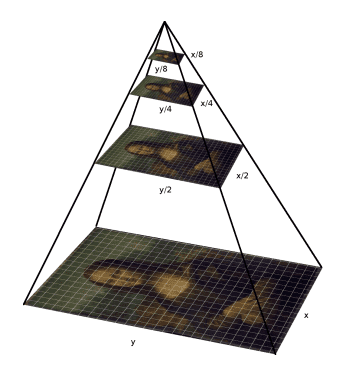
\includegraphics[scale=0.75]{images/detection_chapter/gaussian_pyramid.PNG}
\end{center}
Thanks to image pyramid and sliding windows, we can consider a rectangle at various locations and various scales of the input image. The problem with this procedure are the different bounding boxes surrounding the same object. To deal with this issue, we apply non-maxima suppression. This method allows to maintain only the stronger bounding box, eliminating the extraneous ones. Consider the set P of all the predicted bounding boxes, comprehensive of the confidence score and the overlap threshold, the non-maxima suppression approach goes as follow:
\begin{enumerate}
    \item Delete from P the bounding box S with the top confidence score, and add it to a list F, initially empty, representing the predictions that we maintain
    \item Compute IoU between S and any other prediction T present in P. Delete T from P only if each resulting IoU is greater than the overlap threshold.
    \item If P is empty return F and stop, otherwise compute step 1 and step 2
\end{enumerate}
\begin{center}
    \begin{figure}[!htb]
        \begin{minipage}{0.5\textwidth}
            \centering
            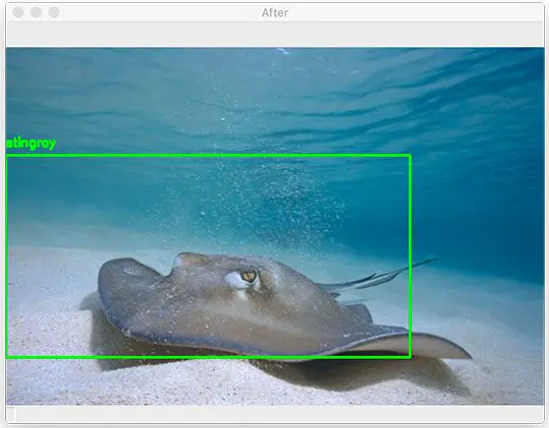
\includegraphics[scale=0.5]{images/detection_chapter/after_nms.PNG}
        \end{minipage}
        \begin{minipage}{0.5\textwidth}
            \centering
            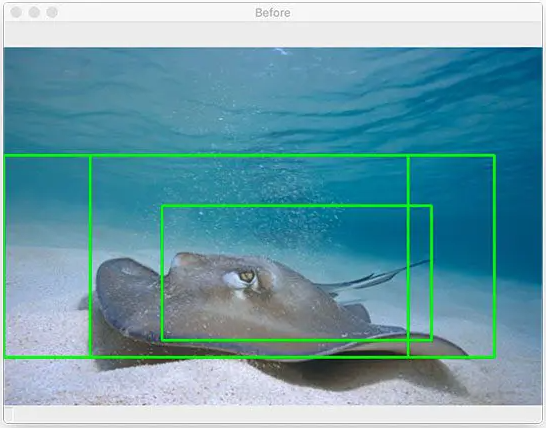
\includegraphics[scale=0.5]{images/detection_chapter/before_nms.PNG} 
        \end{minipage}
    \end{figure}
\end{center}
Finally, the last step applied is one that is used to remove occlusions. Such step consist of removing the bounding boxes obtained after Non Maxima Suppression that may not contain an hand.
In particular such step consist of, for each bounding box after Non Maxima Suppresion (notice that, this step can be only applied if the orginal image was not a grayscale image) : 
\begin{enumerate}
    \item Get the ROI identified by selected bounding boxes
    \item Convert the ROI to an image into the color space YCrCb
    \item Threshold the ROI with a certain range of colors (range of the skin color)
    \item Compute \( percentage = \frac{\#pixels\:equal\:to\:255\:in\:thresholded\:image}{image\:size}\)
    \item Reject the bounding box if \( percentage \leq threshold \)
\end{enumerate}
The detection task is quite time-consuming, principally do to the sliding window method. As future work, we suggest to reduce the computational complexity by using an alternative approach of sliding window.